\documentclass[11pt,letterpaper]{article}
\PassOptionsToPackage{hyphens}{url}
\usepackage[margin=.83in,top=.8in,bottom=.8in,headheight=15pt]{geometry}
\usepackage[T1]{fontenc}
\usepackage{lmodern,amsmath,amssymb,mathtools,bm,booktabs,array,graphicx,tikz}
\usetikzlibrary{arrows.meta,positioning,calc,decorations.pathreplacing,patterns}
\definecolor{ink}{HTML}{17344D}\definecolor{accent}{HTML}{087E8B}\definecolor{pale}{HTML}{EDF5F5}\definecolor{gold}{HTML}{AD6B19}
\providecommand{\dd}{\,\mathrm{d}}\providecommand{\R}{\mathbb{R}}
\providecommand{\E}{\mathbb{E}}\providecommand{\Var}{\operatorname{Var}}
\providecommand{\Cov}{\operatorname{Cov}}\providecommand{\diag}{\operatorname{diag}}
\providecommand{\norm}[1]{\left\lVert#1\right\rVert}
\providecommand{\abs}[1]{\left|#1\right|}
\usepackage{microtype,hyperref,fancyhdr,enumitem,amsthm,sectsty,needspace}
\allsectionsfont{\raggedright}
\hypersetup{colorlinks=true,linkcolor=ink,urlcolor=accent,pdfauthor={Zan Ahmad},pdftitle={A periodically forced circulation / Lecture notes}}
\setlength{\parindent}{0pt}\setlength{\parskip}{6pt}\linespread{1.07}
\setlist{itemsep=3pt,topsep=4pt,leftmargin=*}
\emergencystretch=2em\clubpenalty=10000\widowpenalty=10000
\pagestyle{fancy}\fancyhf{}\fancyhead[L]{\small Computational Cardiology}\fancyhead[R]{\small Lecture 2}
\fancyfoot[L]{\footnotesize Zan Ahmad}\fancyfoot[R]{\footnotesize\thepage}\renewcommand{\headrulewidth}{.3pt}
\newtheorem{proposition}{Proposition}\newtheorem{theorem}{Theorem}\newtheorem{lemma}{Lemma}
\theoremstyle{definition}\newtheorem{definition}{Definition}\newtheorem{example}{Example}
\numberwithin{equation}{section}
\begin{document}
{\small\scshape Computational Cardiology\hfill Lecture 2}\par\medskip
{\raggedright\hyphenpenalty=10000\exhyphenpenalty=10000\LARGE\bfseries\color{ink} A periodically forced circulation\par}\medskip
{\small Lecture notes}\par\bigskip
The six-compartment model combines a closed volume balance with a periodically changing constitutive law. Pressure is therefore neither conserved nor generally stationary. The useful invariants are obtained from the stored volumes, while periodic behavior is described by comparing states at the same cardiac phase.

\section{The six-region initial-value problem}
\hypertarget{note-the-six-region-initial-value-problem}{}\label{note:the-six-region-initial-value-problem}
{\small \href{slides.html\#frame=a-closed-six-region-network\&step=1}{Slides for this section}}\par
A baseline is a fully specified experiment, not merely a familiar filename. Record the model topology, initial state, parameter values, cardiac rate, time step, duration and numerical method. The new companion uses six storage regions in the order LV, systemic artery, systemic vein, RV, pulmonary artery and pulmonary vein. Its links are four directed ideal valves followed by systemic and pulmonary vascular beds. The boundary is closed: no external reservoir supplies or removes blood.

The implementation follows the source's compartment and implicit-valve methodology. The recovered historical initializer sets systemic resistance to 8 mmHg min/L. This teaching baseline uses 17.86, a documented illustrative choice associated with the book baseline. The two numbers are not interchangeable provenance labels. When code and a printed example disagree, first inspect parameters and initialization before diagnosing numerical failure. A matched method with different parameters should generally produce different trajectories.

In the fixed-rate experiment, the rate is fixed at 80 beats/min, systemic resistance does not change, and there is no pressure-feedback action. The local hydraulic component also contains parameter definitions used by the later feedback lesson, but this driver calls only the compliance and pressure-step routines. This restricted experiment lets us audit storage, units and startup before introducing a controller whose errors could otherwise obscure those mechanisms.

Let $x_i=V_i-V_{d,i}$ denote stressed volume. For a prescribed phase $\phi$, pressures are recovered from $P_i=x_i/C_i(\phi)$. With $C_i(\phi)>0$, this is an invertible change of state coordinates. The dynamical system is
\[
 \dot x=Bq(P),\qquad P=D_C(\phi)^{-1}x,\qquad \dot\phi=F,
\]
when hydraulic time is measured in minutes. The phase must accompany the pressures whenever the ventricular compliances vary.
\section{Pressure--volume coordinates and cardiac phase}
\hypertarget{note-pressure-volume-coordinates-and-cardiac-phase}{}\label{note:pressure-volume-coordinates-and-cardiac-phase}
{\small \href{slides.html\#frame=stored-volumes-as-state-variables\&step=1}{Slides for this section}}\par
Pressures are in mmHg and volumes are in liters. Each region obeys $V=V_d+CP$, where Vd is its unstressed volume and P is pressure relative to the model's fixed exterior reference. The four vascular compliances are constant. Both ventricular compliances change with one shared phase. A pressure vector alone therefore does not determine volume unless the phase and compliance law are also supplied. Equivalently, a volume-based state needs the same law to recover pressure.

The interface records time in seconds because a heartbeat is convenient to inspect on that scale. Hydraulic resistance has units mmHg min/L and flow has L/min. A hydraulic step must therefore use elapsed seconds divided by 60. The baseline step is 0.001875 s, or 0.00003125 min. At 80 beats/min the cycle lasts 0.75 s, giving 400 nominal steps per beat. These are different units describing one interval; passing the seconds value directly to a minute-based balance multiplies transferred volume by 60.

Initialization is explicit. At phase zero, ventricular compliances are 0.0146 and 0.0365 L/mmHg. Initial pressures are [5,80,2,2,8,5] mmHg. Unstressed volumes are [0.027,0.825,0,0.027,0.0382,0] L. The remaining compliances are 0.00175, 1.75, 0.00412 and 0.08 L/mmHg for systemic artery, systemic vein, pulmonary artery and pulmonary vein. These values determine every initial compartment volume algebraically.

\[
V_i(t)=V_{d,i}+C_i(\phi(t))P_i(t)
\]
V and Vd are liters, C is L/mmHg, P is mmHg.

\[
\phi(t_s)=F t_s/60
\]
For this fixed-rate baseline, both ventricles use exactly this phase.

The initialized total follows directly from the supplied vectors:
\[
 V_{\rm tot}=\sum_i V_{d,i}+\sum_i C_i(0)P_i(0)=5.13616\ \mathrm L.
\]
At $F=80\ \mathrm{min}^{-1}$ the beat period is $T_b=60/F=0.75$ s. A $0.001875$ s step corresponds to $h=3.125\times10^{-5}$ min and advances phase by $Fh=1/400$ cycle.

\paragraph{Calculation.} Reconstruct all initial volumes from the listed phase-zero state.

LV: 0.027 + 0.0146\ensuremath{\times}5 = 0.100 L; systemic artery: 0.825 + 0.00175\ensuremath{\times}80 = 0.965 L.

Systemic vein: 1.75\ensuremath{\times}2 = 3.500 L; RV: 0.027 + 0.0365\ensuremath{\times}2 = 0.100 L.

Pulmonary artery: 0.0382 + 0.00412\ensuremath{\times}8 = 0.07116 L; pulmonary vein: 0.08\ensuremath{\times}5 = 0.400 L.

Summing gives initial total blood volume 5.13616 L.

The total follows from initialization; it is not an independently fitted patient measurement.
\section{Periodic forcing and the return map}
\hypertarget{note-periodic-forcing-and-the-return-map}{}\label{note:periodic-forcing-and-the-return-map}
{\small \href{slides.html\#frame=a-periodically-forced-state-panel-1\&step=1}{Slides for this section}}\par
Each compartment obeys inflow minus outflow equals its volume-change rate. Ventricular contraction changes compliance and redistributes blood through pressure-driven valves. A compartment may gain volume while another loses it. Total volume can stay constant even when pressures and individual volumes vary strongly. ``Conserved'' therefore does not mean that every plotted line is horizontal.

The first figure shows three pressures and the two ventricular volumes through the full 15-second startup. Initial values were prescribed for reproducibility, rather than solved as a periodic steady state. The first beat need not resemble a later beat. Repeated cycles become more similar as the state redistributes, but whether the run is sufficiently close to periodic depends on the observable, tolerance and chosen parameters. Inspecting only the final point hides within-cycle differences.

Compare two windows at the same cardiac phase. At 80 beats/min, shift one window by 0.75 s and compare pressures component by component. The companion samples the last two complete cycles on a common phase-aligned grid. In the supplied calculation their maximum pressure difference is approximately 0.073 mmHg. That number measures remaining cycle-to-cycle change for this run. It is not a time-discretization error estimate or a laboratory validation result.

Denote the one-beat solution map at a fixed starting phase by $\mathcal P$. A periodic state satisfies
\[
 x_* = \mathcal P(x_*),\qquad \boldsymbol1^{\mathsf T}x_* = V_{\rm tot}-\sum_iV_{d,i}.
\]
A trajectory can approach this fixed point while retaining large within-beat oscillations. A useful residual is $\|P(t+T_b)-P(t)\|_\infty$ at matched phases. It measures departure from periodicity, not the error of the numerical trajectory relative to the differential equations.
\begin{center}\begin{minipage}{.98\linewidth}\centering
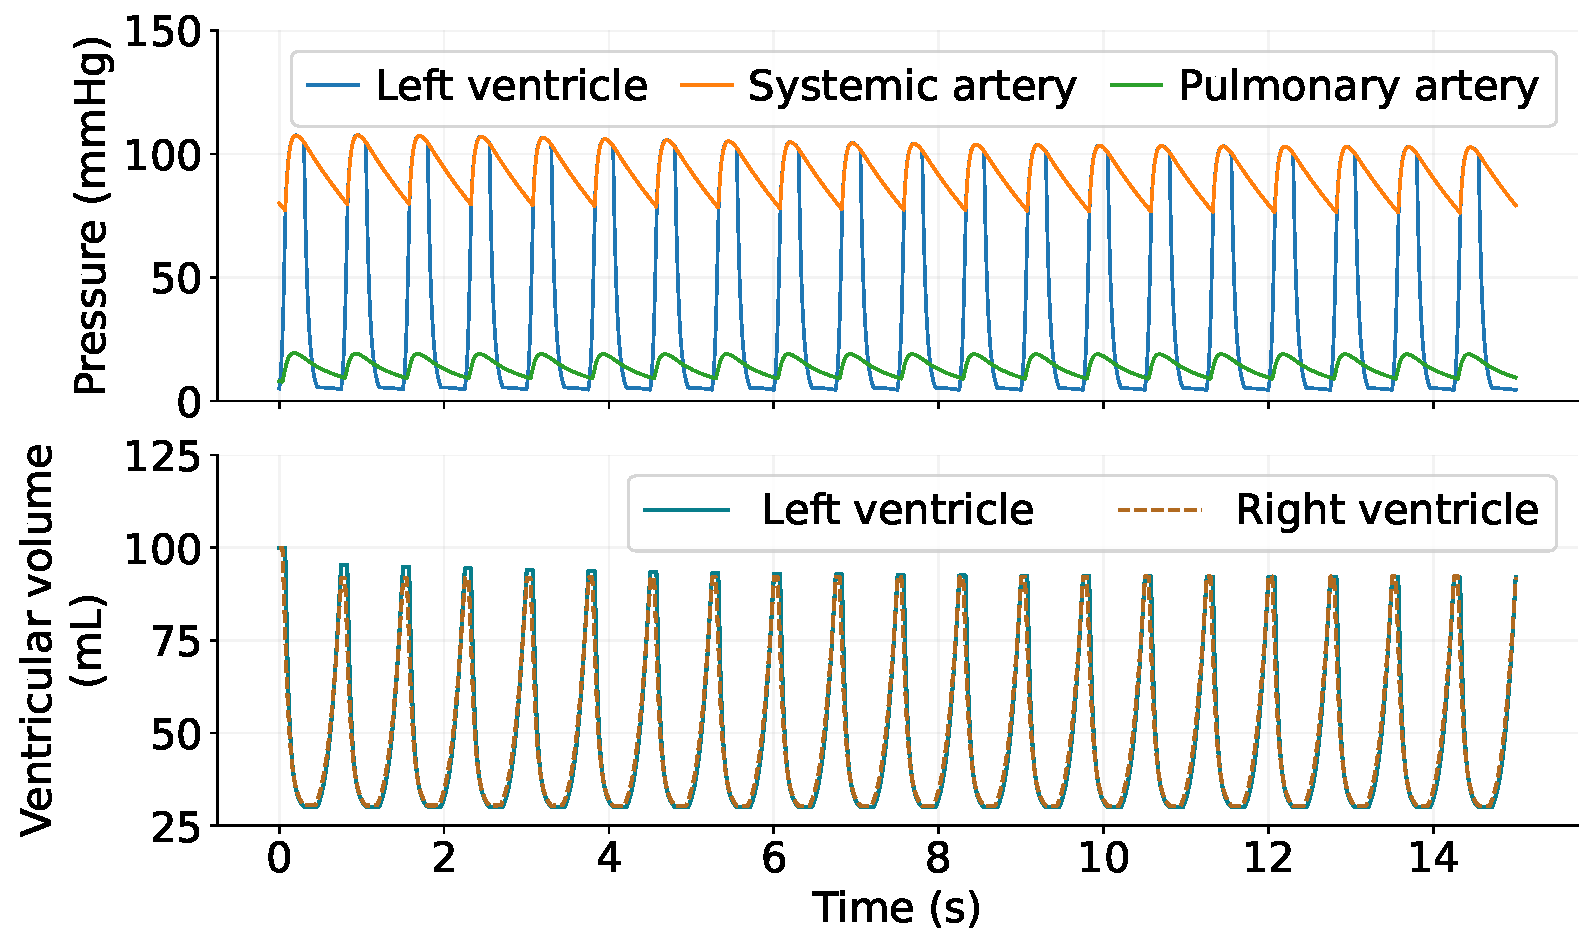
\includegraphics[width=.96\linewidth,height=.57\textheight,keepaspectratio]{baseline-state.pdf}\par\smallskip
{\small New fixed-rate six-compartment calculation: F=\allowbreak{}80 beats/min, Rs=\allowbreak{}17.86 mmHg min/L, 15 s, step 0.001875 s. Individual pressures and volumes change during startup and pumping.}
\end{minipage}\end{center}
\section{The discrete volume invariant}
\hypertarget{note-the-discrete-volume-invariant}{}\label{note:the-discrete-volume-invariant}
{\small \href{slides.html\#frame=sum-the-compartment-equations\&step=1}{Slides for this section}}\par
Write one volume balance per storage region. For a link carrying Q from region i to j, the two balances contain \ensuremath{-}Q and +Q. Summing all six cancels every link regardless of whether its flow changes during the beat. With fixed unstressed volumes, total volume is the sum of Vd + C P. The discrete pressure solver is constructed to preserve the same identity between accepted steps. This is stronger evidence than seeing a plausible waveform, but it checks only the stated account.

Always reconstruct volume using the compliance at the saved phase. Reusing phase-zero ventricular compliance with later pressures creates a false drift signal because it applies the wrong pressure-volume law. The companion deliberately evaluates that wrong audit as a teaching counterexample. It produces an apparent drift exceeding 2 L, while the correct audit stays within about 1.2e\ensuremath{-}12 L in the supplied calculation. The bad diagnostic does not prove the pressure solver leaked; it proves the diagnostic used inconsistent states.

The second figure displays both the absolute total and the tiny difference from its initial value. The drift panel uses nanoliters so the small rounding residual is visible without implying a physiologically meaningful variation. Report the scale and maximum absolute residual; an automatically rescaled vertical axis can make a floating-point effect look like a large physical oscillation. The compartment sum provides a direct reconstruction of the conserved total.

\[
\frac{d}{dt}\sum_{i=1}^{6}V_i=\sum_{i=1}^{6}(Q_{{\rm in},i}-Q_{{\rm out},i})=0
\]
Every modeled transfer is internal to the closed boundary.

\[
\varepsilon_V(t)=\sum_i[V_{d,i}+C_i(\phi(t))P_i(t)]-V_{\rm total}(0)
\]
Use matched pressures, phase and compliances at every saved time.

Summing the discrete balances gives
\[
 \boldsymbol1^{\mathsf T}\bigl(D_C^{n+1}P^{n+1}-D_C^nP^n\bigr)
   =h\boldsymbol1^{\mathsf T}Bq^{n+1}=0.
\]
Replacing $D_C^{n+1}$ by $D_C^0$ in a diagnostic changes the quantity being measured. The resulting discrepancy includes $\sum_i[C_i(0)-C_i(t)]P_i(t)$, which need not be small even when the true invariant is preserved exactly.
\begin{center}\begin{minipage}{.98\linewidth}\centering
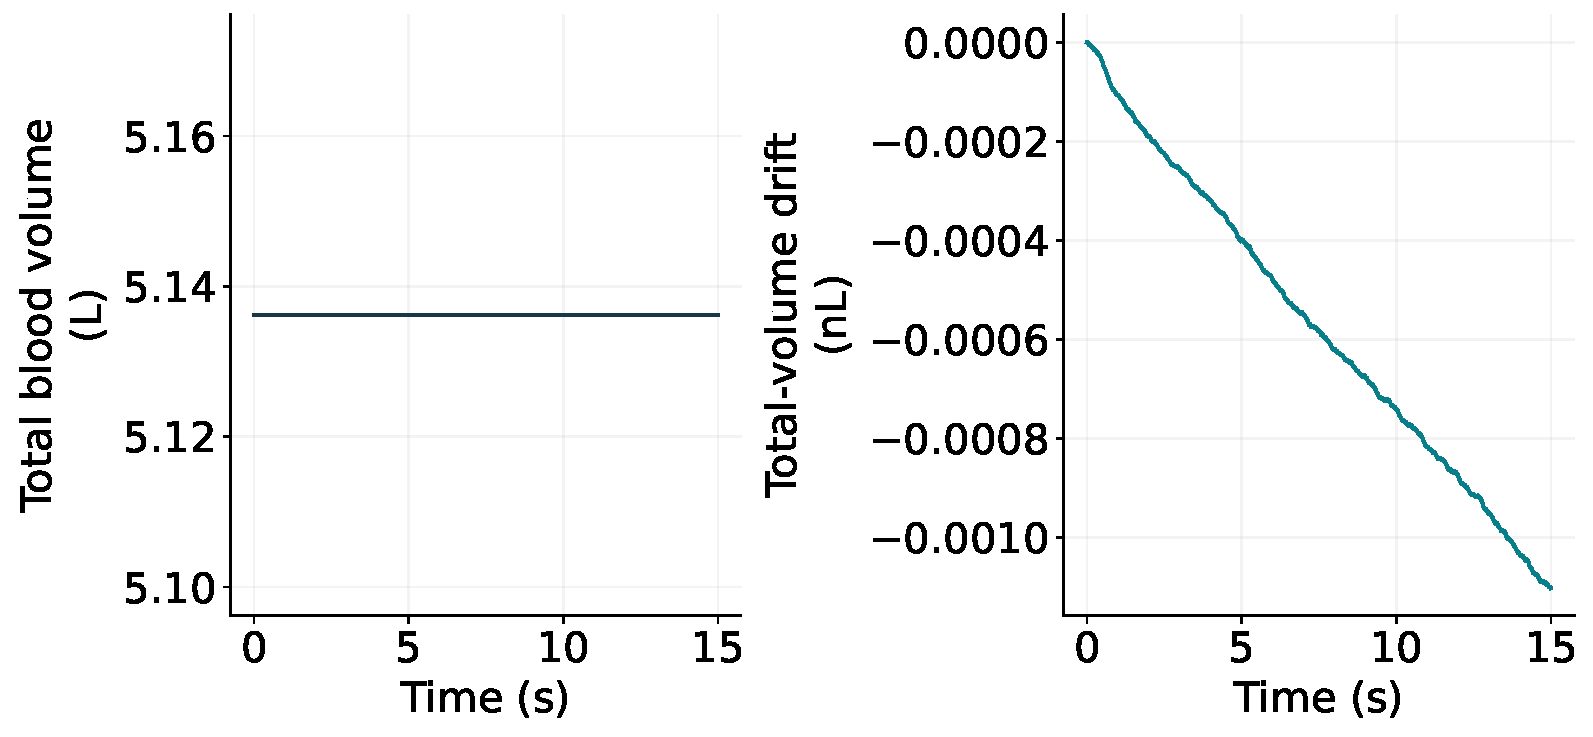
\includegraphics[width=.96\linewidth,height=.57\textheight,keepaspectratio]{volume-audit.pdf}\par\smallskip
{\small The initialized total is 5.13616 L. The right panel shows numerical drift in nanoliters, distinct from physiological volume redistribution.}
\end{minipage}\end{center}
\section{Transient decay and discretization error}
\hypertarget{note-transient-decay-and-discretization-error}{}\label{note:transient-decay-and-discretization-error}
{\small \href{slides.html\#frame=phase-aligned-comparison\&step=1}{Slides for this section}}\par
A startup transient compares the evolving solution at different cycles under the same parameters. Conservation drift measures a violated closed-volume account. Time-step error compares different numerical resolutions at the same physical time and with the same model and initial state. None is interchangeable with the others. A perfectly conserved trajectory can still be inaccurate, and an accurate transient need not yet be periodic.

The hydraulic update is implicit backward Euler with valve-state consistency. It is not explicit Euler merely because the program has a time loop. New pressures are found by solving coupled balances using new compliances; guessed valve states are checked against those solved pressure differences. The returned balance residual measures satisfaction of the coupled equations.

The refinement comparison uses two short runs at a common 1.5-second endpoint with steps 0.001875 and 0.0009375 s. Their largest pressure difference is about 0.031 mmHg. A pairwise difference shows sensitivity to refinement; it does not establish an asymptotic order or certify convergence by itself. An asymptotic order requires a refinement sequence and an appropriate reference. Changing the time step must not simultaneously change resistance, initialization or the duration being compared.

These discrepancies compare different mathematical objects:
\[
 \begin{aligned}
 r_{\rm per}(t)&=\|P_h(t+T_b)-P_h(t)\|_\infty,\\
 r_V(t)&=\left|\sum_iV_{i,h}(t)-V_{\rm tot}(0)\right|,\\
 d_h(t)&=\|P_h(t)-P_{h/2}(t)\|_\infty.
 \end{aligned}
\]
A small $r_V$ follows from an algebraic invariant of the method and does not imply a small $d_h$. Likewise, a physical startup transient can produce a large $r_{\rm per}$ in a well-resolved calculation.
\section{Constitutive consistency and parameter dependence}
\hypertarget{note-constitutive-consistency-and-parameter-dependence}{}\label{note:constitutive-consistency-and-parameter-dependence}
{\small \href{slides.html\#frame=resistance-changes-the-dynamics\&step=1}{Slides for this section}}\par
Run the supplied baseline and record its initial total, maximum volume residual, maximum compartment-balance residual, minimum stored volume and minimum forward valve flow. Identify the units of every quantity. Ideal-valve flow is nonnegative in its declared forward direction; the two vascular beds remain open resistors and their signs should be interpreted using pressure differences. Clipping arbitrary outputs after the solve would hide a change of model and can destroy balance.

Changing $R_s$ changes the vector field because $q_s=(P_{sa}-P_{sv})/R_s$. It need not change the conserved total, which follows from the network boundary. Conservation is therefore compatible with substantially different trajectories. The rate, resistance, initial state and constitutive law must all remain fixed when attributing a difference to numerical resolution.
\bigskip
\section*{Exercises}
\par\noindent\begin{minipage}{\linewidth}
\subsection*{A2-1. Reconstruct a smaller state}
Two closed storage regions have Vd=\allowbreak{}[0.03,0.20] L, C=\allowbreak{}[0.02,0.10] L/mmHg and P=\allowbreak{}[10,4] mmHg.

\textbf{a} Calculate both stored volumes and their total.

\end{minipage}\par\medskip
\textbf{b} A 3 L/min transfer moves from region 1 to 2 for 0.3 s. Compute the transferred volume.

\textbf{c} Compute the new volumes and check the total.

\par\noindent\begin{minipage}{\linewidth}
\subsection*{A2-2. Classify a diagnostic}
Run A preserves total volume at 5.1 L while successive beat shapes change. Run B shows a steadily changing total although it has no external source.

\textbf{a} Which observation is compatible with a startup transient?

\end{minipage}\par\medskip
\textbf{b} Give two checks before concluding Run B has a solver leak.

\textbf{c} How would you assess time-step error independently of cycle change?

\par\noindent\begin{minipage}{\linewidth}
\subsection*{A2-3. Repair a unit and provenance record}
A report uses h=\allowbreak{}0.003 s in an equation whose flows are L/min, and labels a run with Rs=\allowbreak{}17.86 as an unchanged reproduction of an initializer that uses Rs=\allowbreak{}8.

\textbf{a} Find the correct hydraulic step and the transfer at Q=\allowbreak{}4 L/min.

\end{minipage}\par\medskip
\textbf{b} Rewrite the provenance claim accurately.

\textbf{c} Would a passing total-volume test detect the wrong time unit automatically?

\section*{References}
\noindent\begin{minipage}{\linewidth}
Zan Ahmad, Advanced Topics in Computational Cardiology syllabus, Fall 2024. PDF pages 1--2.

\end{minipage}\par\medskip
\noindent\begin{minipage}{\linewidth}
Hoppensteadt and Peskin, Modeling and Simulation in Medicine and the Life Sciences, second edition. Printed pages 55--58; supplied PDF pages 68--71.

\end{minipage}\par\medskip
\end{document}
